
% !TeX root=arXiv.tex
% !TEX TS-program = pdfLatex

%%%%%%%%%%%%%%%%%%%%% EXPERIMENTS %%%%%%%%%%%%%%%%%%%%%%%%%%%%%%%%%%%%%
\section{Experiments}\label{sec.4}

To evaluate our proposed method, we compare it with the state-of-the art methods, as well as an informative baseline.

\subsection{Datasets}\label{sec.4.1}

\begin{figure*}
\scalebox{.4}
{
\begin{tikzpicture}

		\node [scale=2] (strong) {\textit{strong}}; 
	\node [scale=2, right=31cm of strong] (weak) {\textit{weak}};
	\path [draw, line width=3, <->, blue] (strong.south west) -- (weak.south east);

	% attr1
	\node [below=0.5cm of strong] (attr1im1) {
\includegraphics[width=4cm, height=4cm]{spectrum/attr1/im1.jpg}};
	\node (attr1name) [scale=2, left=0.5cm of attr1im1] {Smile};
	\node [right=0.5cm of attr1im1] (attr1im2) {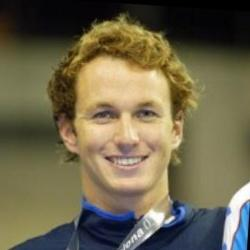
\includegraphics[width=4cm, height=4cm]{spectrum/attr1/im2.jpg}};
	\node [right=0.5cm of attr1im2] (attr1im3) {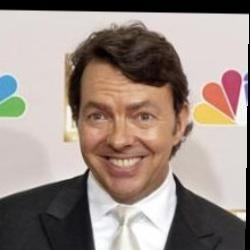
\includegraphics[width=4cm, height=4cm]{spectrum/attr1/im3.jpg}};
	\node [right=0.5cm of attr1im3] (attr1im4) {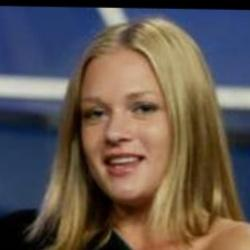
\includegraphics[width=4cm, height=4cm]{spectrum/attr1/im4.jpg}};
	\node [right=0.5cm of attr1im4] (attr1im5) {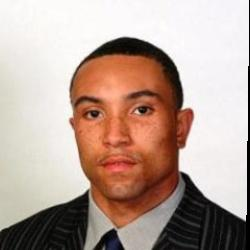
\includegraphics[width=4cm, height=4cm]{spectrum/attr1/im5.jpg}};
	\node [right=0.5cm of attr1im5] (attr1im6) {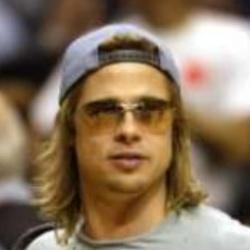
\includegraphics[width=4cm, height=4cm]{spectrum/attr1/im6.jpg}};
	\node [right=0.5cm of attr1im6] (attr1im7) {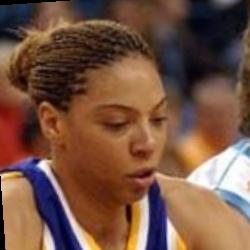
\includegraphics[width=4cm, height=4cm]{spectrum/attr1/im7.jpg}};
	\node [right=0.5cm of attr1im7] (attr1im8) {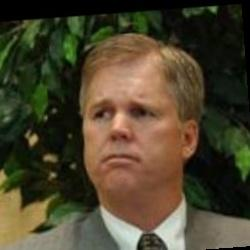
\includegraphics[width=4cm, height=4cm]{spectrum/attr1/im8.jpg}};

	% attr2
	\node [below=0.5cm of attr1im1] (attr2im1) {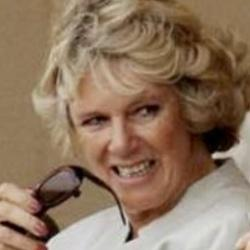
\includegraphics[width=4cm, height=4cm]{spectrum/attr2/im1.jpg}};
	\node (attr2name) [scale=2, left=0.5cm of attr2im1] {Young};
	\node [right=0.5cm of attr2im1] (attr2im2) {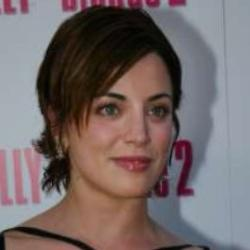
\includegraphics[width=4cm, height=4cm]{spectrum/attr2/im2.jpg}};
	\node [right=0.5cm of attr2im2] (attr2im3) {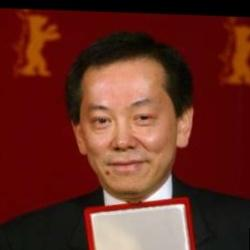
\includegraphics[width=4cm, height=4cm]{spectrum/attr2/im3.jpg}};
	\node [right=0.5cm of attr2im3] (attr2im4) {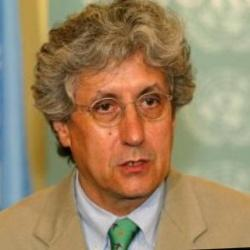
\includegraphics[width=4cm, height=4cm]{spectrum/attr2/im4.jpg}};
	\node [right=0.5cm of attr2im4] (attr2im5) {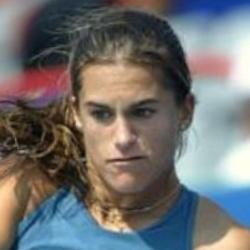
\includegraphics[width=4cm, height=4cm]{spectrum/attr2/im5.jpg}};
	\node [right=0.5cm of attr2im5] (attr2im6) {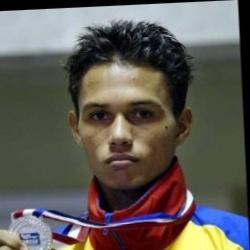
\includegraphics[width=4cm, height=4cm]{spectrum/attr2/im6.jpg}};
	\node [right=0.5cm of attr2im6] (attr2im7) {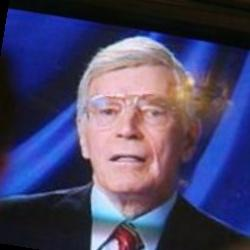
\includegraphics[width=4cm, height=4cm]{spectrum/attr2/im7.jpg}};
	\node [right=0.5cm of attr2im7] (attr2im8) {
\includegraphics[width=4cm, height=4cm]{spectrum/attr2/im8.jpg}};

	% attr3
	\node [below=0.5cm of attr2im1] (attr3im1) {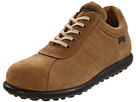
\includegraphics[width=4cm, height=3cm]{spectrum/attr3/im1.jpg}};
	\node (attr3name) [scale=2, left=0.5cm of attr3im1] {Comfort};
	\node [right=0.5cm of attr3im1] (attr3im2) {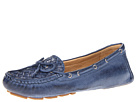
\includegraphics[width=4cm, height=3cm]{spectrum/attr3/im2.jpg}};
	\node [right=0.5cm of attr3im2] (attr3im3) {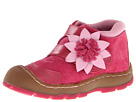
\includegraphics[width=4cm, height=3cm]{spectrum/attr3/im3.jpg}};
	\node [right=0.5cm of attr3im3] (attr3im4) {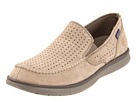
\includegraphics[width=4cm, height=3cm]{spectrum/attr3/im4.jpg}};
	\node [right=0.5cm of attr3im4] (attr3im5) {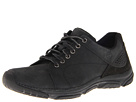
\includegraphics[width=4cm, height=3cm]{spectrum/attr3/im5.jpg}};
	\node [right=0.5cm of attr3im5] (attr3im6) {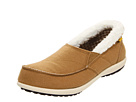
\includegraphics[width=4cm, height=3cm]{spectrum/attr3/im6.jpg}};
	\node [right=0.5cm of attr3im6] (attr3im7) {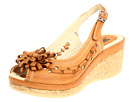
\includegraphics[width=4cm, height=3cm]{spectrum/attr3/im7.jpg}};
	\node [right=0.5cm of attr3im7] (attr3im8) {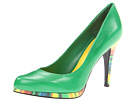
\includegraphics[width=4cm, height=3cm]{spectrum/attr3/im8.jpg}};

	% attr4
	\node [below=0.5cm of attr3im1] (attr4im1) {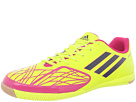
\includegraphics[width=4cm, height=3cm]{spectrum/attr4/im1.jpg}};
	\node (attr4name) [scale=2, left=0.5cm of attr4im1] {Sporty};
	\node [right=0.5cm of attr4im1] (attr4im2) {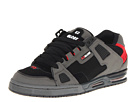
\includegraphics[width=4cm, height=3cm]{spectrum/attr4/im2.jpg}};
	\node [right=0.5cm of attr4im2] (attr4im3) {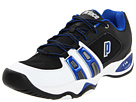
\includegraphics[width=4cm, height=3cm]{spectrum/attr4/im3.jpg}};
	\node [right=0.5cm of attr4im3] (attr4im4) {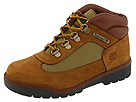
\includegraphics[width=4cm, height=3cm]{spectrum/attr4/im4.jpg}};
	\node [right=0.5cm of attr4im4] (attr4im5) {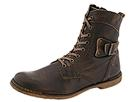
\includegraphics[width=4cm, height=3cm]{spectrum/attr4/im5.jpg}};
	\node [right=0.5cm of attr4im5] (attr4im6) {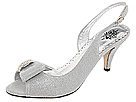
\includegraphics[width=4cm, height=3cm]{spectrum/attr4/im6.jpg}};
	\node [right=0.5cm of attr4im6] (attr4im7) {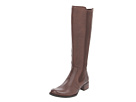
\includegraphics[width=4cm, height=3cm]{spectrum/attr4/im7.jpg}};
	\node [right=0.5cm of attr4im7] (attr4im8) {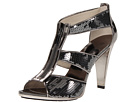
\includegraphics[width=4cm, height=3cm]{spectrum/attr4/im8.jpg}};

	% attr5
	\node [below=0.5cm of attr4im1] (attr5im1) {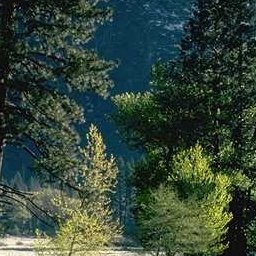
\includegraphics[width=4cm, height=4cm]{spectrum/attr5/im1.jpg}};
	\node (attr5name) [scale=2, left=0.5cm of attr5im1] {Natural};
	\node [right=0.5cm of attr5im1] (attr5im2) {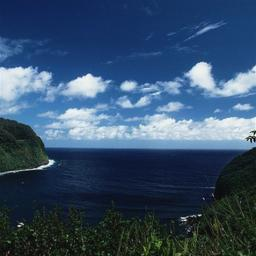
\includegraphics[width=4cm, height=4cm]{spectrum/attr5/im2.jpg}};
	\node [right=0.5cm of attr5im2] (attr5im3) {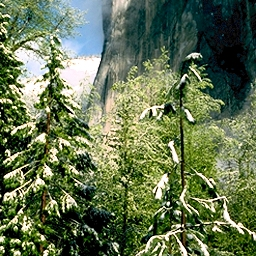
\includegraphics[width=4cm, height=4cm]{spectrum/attr5/im3.jpg}};
	\node [right=0.5cm of attr5im3] (attr5im4) {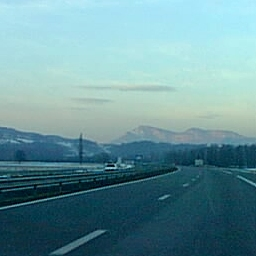
\includegraphics[width=4cm, height=4cm]{spectrum/attr5/im4.jpg}};
	\node [right=0.5cm of attr5im4] (attr5im5) {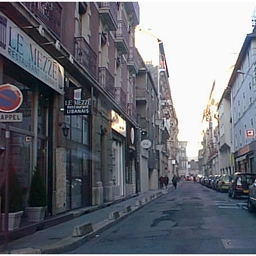
\includegraphics[width=4cm, height=4cm]{spectrum/attr5/im5.jpg}};
	\node [right=0.5cm of attr5im5] (attr5im6) {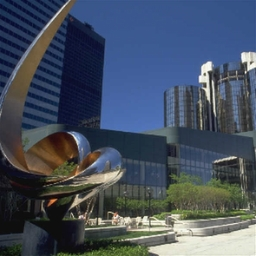
\includegraphics[width=4cm, height=4cm]{spectrum/attr5/im6.jpg}};
	\node [right=0.5cm of attr5im6] (attr5im7) {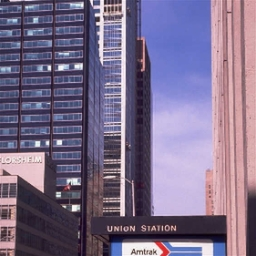
\includegraphics[width=4cm, height=4cm]{spectrum/attr5/im7.jpg}};
	\node [right=0.5cm of attr5im7] (attr5im8) {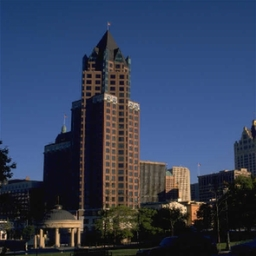
\includegraphics[width=4cm, height=4cm]{spectrum/attr5/im8.jpg}};

	% attr6
	\node [below=0.5cm of attr5im1] (attr6im1) {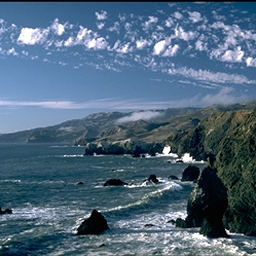
\includegraphics[width=4cm, height=4cm]{spectrum/attr6/im1.jpg}};
	\node (attr6name) [scale=2, left=0.5cm of attr6im1] {Open};
	\node [right=0.5cm of attr6im1] (attr6im2) {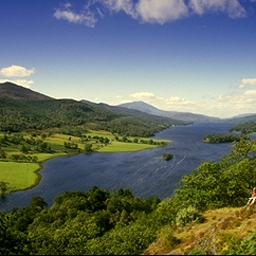
\includegraphics[width=4cm, height=4cm]{spectrum/attr6/im2.jpg}};
	\node [right=0.5cm of attr6im2] (attr6im3) {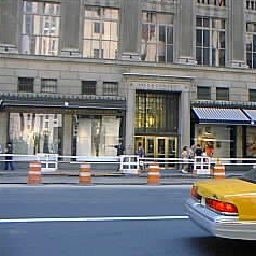
\includegraphics[width=4cm, height=4cm]{spectrum/attr6/im3.jpg}};
	\node [right=0.5cm of attr6im3] (attr6im4) {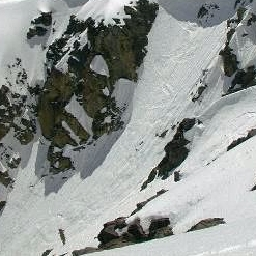
\includegraphics[width=4cm, height=4cm]{spectrum/attr6/im4.jpg}};
	\node [right=0.5cm of attr6im4] (attr6im5) {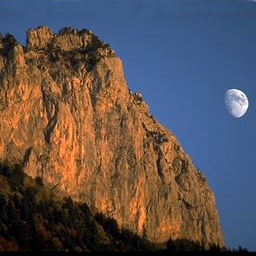
\includegraphics[width=4cm, height=4cm]{spectrum/attr6/im5.jpg}};
	\node [right=0.5cm of attr6im5] (attr6im6) {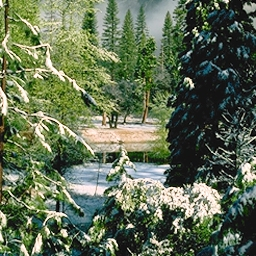
\includegraphics[width=4cm, height=4cm]{spectrum/attr6/im6.jpg}};
	\node [right=0.5cm of attr6im6] (attr6im7) {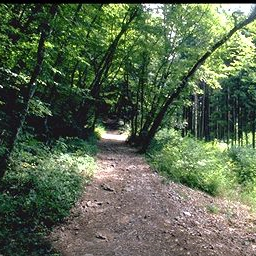
\includegraphics[width=4cm, height=4cm]{spectrum/attr6/im7.jpg}};
	\node [right=0.5cm of attr6im7] (attr6im8) {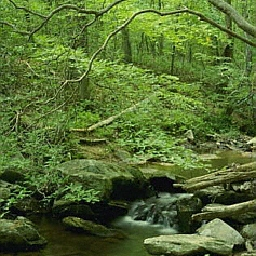
\includegraphics[width=4cm, height=4cm]{spectrum/attr6/im8.jpg}};

	% attr7
	\node [below=0.5cm of attr6im1] (attr7im1) {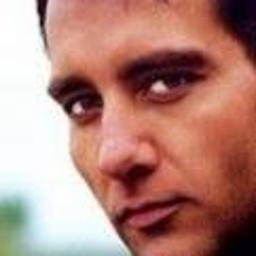
\includegraphics[width=4cm, height=4cm]{spectrum/attr7/im1.jpg}};
	\node (attr7name) [scale=2, left=0.5cm of attr7im1] {Forehead};
	\node [right=0.5cm of attr7im1] (attr7im2) {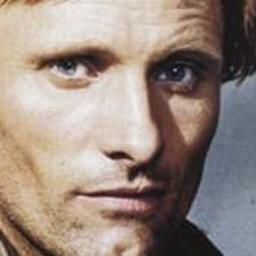
\includegraphics[width=4cm, height=4cm]{spectrum/attr7/im2.jpg}};
	\node [right=0.5cm of attr7im2] (attr7im3) {\includegraphics[width=4cm, height=4cm]{spectrum/attr7/im3.jpg}};
	\node [right=0.5cm of attr7im3] (attr7im4) {\includegraphics[width=4cm, height=4cm]{spectrum/attr7/im4.jpg}};
	\node [right=0.5cm of attr7im4] (attr7im5) {\includegraphics[width=4cm, height=4cm]{spectrum/attr7/im5.jpg}};
	\node [right=0.5cm of attr7im5] (attr7im6) {\includegraphics[width=4cm, height=4cm]{spectrum/attr7/im6.jpg}};
	\node [right=0.5cm of attr7im6] (attr7im7) {\includegraphics[width=4cm, height=4cm]{spectrum/attr7/im7.jpg}};
	\node [right=0.5cm of attr7im7] (attr7im8) {\includegraphics[width=4cm, height=4cm]{spectrum/attr7/im8.jpg}};

	% attr8
	\node [below=0.5cm of attr7im1] (attr8im1) {\includegraphics[width=4cm, height=4cm]{spectrum/attr8/im1.jpg}};
	\node (attr8name) [scale=2, left=0.5cm of attr8im1] {Open Eyes};
	\node [right=0.5cm of attr8im1] (attr8im2) {\includegraphics[width=4cm, height=4cm]{spectrum/attr8/im2.jpg}};
	\node [right=0.5cm of attr8im2] (attr8im3) {\includegraphics[width=4cm, height=4cm]{spectrum/attr8/im3.jpg}};
	\node [right=0.5cm of attr8im3] (attr8im4) {\includegraphics[width=4cm, height=4cm]{spectrum/attr8/im4.jpg}};
	\node [right=0.5cm of attr8im4] (attr8im5) {\includegraphics[width=4cm, height=4cm]{spectrum/attr8/im5.jpg}};
	\node [right=0.5cm of attr8im5] (attr8im6) {\includegraphics[width=4cm, height=4cm]{spectrum/attr8/im6.jpg}};
	\node [right=0.5cm of attr8im6] (attr8im7) {\includegraphics[width=4cm, height=4cm]{spectrum/attr8/im7.jpg}};
	\node [right=0.5cm of attr8im7] (attr8im8) {\includegraphics[width=4cm, height=4cm]{spectrum/attr8/im8.jpg}};
\end{tikzpicture}}
\caption{Images sorted according to the strength of their respective attributes.}
\label{figspectrum}
\end{figure*}

To assess the performance of the proposed method, we have evaluated it on all publicly available datasets to our knowledge: \textbf{Zappos50k} \cite{Yu2014} (both coarse and fine-grained versions), \textbf{LFW10} \cite{Sandeep_2014_CVPR} and for the sake of completeness and comparison with previous works on \textbf{PubFig} and \textbf{OSR} datasets of \cite{parikh2011}.

\textbf{UT-Zap50K} \cite{Yu2014} dataset is a collection of images with 4 attributes. This dataset contains two collections: Zappos50k-1 where relative attributes are annotated for coarse pairs where the distinction is relatively easy to make, and Zappos50k-2 where relative attributes are annotated for fine-grained pairs which making the distinction between them is hard according to human annotators.
Zappos50k-1 contains approximately 1500 to 1800 annotated pairs for each attribute. These are divided into 10 train/test splits which are provided alongside the dataset and used in this work. Meanwhile Zappos50k-2 only contains a test set of approximately 4300 pairs, and for training the set of images in Zappos50k-1 is used.
% This dataset consists of two collections, namely UT-Zap50K-1, in which \textit{coarse} relative attributes are compared for image pairs, and UT-Zap50K-2, in which \textit{fine-grained} relative attributes are compared for image pairs.
We have also conducted experiments on the \textbf{LFW-10} \cite{Sandeep_2014_CVPR} dataset. This dataset has 2000 images of people faces and 10 attributes. For each attribute, a random subset of 500 pairs of images have been annotated for each train and test set.
% These two latter datasets have large number of categories, as well as large inter-sample varieties in terms of poses, lighting condition. This makes them quite challenging compared to PubFig and OSR.

\textbf{PubFig} \cite{parikh2011} dataset (a set of public figure faces), consists of 800 facial images of 8 random subjects, with 11 attributes.
\textbf{OSR} \cite{parikh2011} dataset contains 2688 images of outdoor scences in 8 categories, for which 6 relative attributes are defined.
The ordering of the attributes in both PubFig and OSR datasets are annotated in a category level, \ie, all images in a specific category may be ranked higher, equal, or lower than all images in another category, with respect to an attribute. This sometimes causes annotation inconsistencies \cite{Sandeep_2014_CVPR}.
In our experiments we have used the provided train/test split of PubFig and OSR datasets.

% Like the PubFig dataset, relative ranking of attributes for this dataset is annotated in a category level. These two datasets are widely used in the literature, and therefore can provide us a good testbed to compare our results with the previous results acquired by the state-of-the-art methods. 

% In addition to these datasets, we use the \textbf{MNIST} \cite{lecun1998mnist} dataset, to further analyze the properties of our proposed end-to-end model and the obtained feature hierarchy. We have incorporated the class labels of the images as the relative attributes, and used the label values to rank images.
\subsection{Experimental setup}
We train our proposed model (described in Section \ref{sec.3}) for each attribute, separately. While desirable to train multiple attributes at the same time, this is not done due to the nature of the datasets, where for each training pair of images only a certain attribute is annotated.

In all our experiments, for the feature learning and extraction part of the network, we use layer fc7 of VGG-16 model of \cite{verydeep} (the last layer before the probability layer). We initialize their weights using a pretrained model on ILSVRC2014 dataset \cite{ilsvrc2014}. These weights will get fine-tuned as the network learns to predict the relative attributes. The weights $w$ of the ranking layer are initialized using the Xavier method \cite{glorot}, and the bias is initialized to 0.

For training, we use stochastic gradient descent with RMSProp updates and minibatches of size 32 (16 pair of images). In each epoch, we randomly shuffle the training pairs. The number of epochs of training were chosen to reflect the training size. For Zappos50k and LFW10 datasets, we train for 5 and 50 epochs, respectively. For PubFig and OSR datasets, we train for 120 epochs due to the small number of training samples. Also we have added random flipping of the training images as a way to augment the training set on the PubFig and OSR datasets.

\subsection{Baseline}

As a baseline, we have also included results for the RankSVM method (as in \cite{parikh2011}), when the features given to the method are computed from the output of the VGG16 pretrained network on ILSVRC2014. This baseline shows the effect of features fine-tuning, for the task. For each single dataset, we have also compared our results with the best previously reported state-of-the-art approaches. 

\subsection{Results}

Following \cite{parikh2011, Yu2014, Sandeep_2014_CVPR}, we report the accuracy in terms of the percentage of correctly ordered pairs. For our proposed method, we report the mean accuracy over 3 separate runs. For a complete report on the results including the standard deviation of the results see supplementary materials.

Table \ref{tab:osr} shows our results on OSR dataset. Our method outperforms the baseline and the state-of-the-art on this dataset, on all attributes except for `Natural' attribute, where the baseline outperforms our method with a small margin. One possible cause of this could be that the pretrained network of the baseline is still appropriate for this dataset, since the dataset contains natural images. This is a relatively easy dataset, and we would assume that it is not able show the ability of our method to learn features.

%%%%%%%%%%%%%%%%%%%%%% OSR RESULTS %%%%%%%%%%%%%%%%%%%%%
\begin{table*}[t!]
\caption{Results for the OSR dataset}
\centering
\resizebox{2\columnwidth}{!}{
\begin{tabular}{l| c | c | c | c | c | c | c }
\textbf{Method} & \textbf{Natural} & \textbf{Open} &  \textbf{Prespective} & \textbf{Large Size} & \textbf{Diag} & \textbf{ClsDepth} & \textbf{Mean}\\ \hline
 Relative Attributes~\cite{parikh2011} &  95.03 & 90.77 & 86.73 & 86.23 & 86.50 & 87.53 & 88.80 \\
 Relative Forest~\cite{Li2013} & 95.24 & 92.39 & 87.58 & 88.34 & 89.34 & 89.54 & 90.41 \\
 Fine-grained Comparison~\cite{Yu2014} & 95.70 & 94.10 & 90.43 & 91.10 & 92.43 & 90.47 & 92.37 \\
 VGG16-fc7 (baseline) & 97.98 & 87.82 & 89.01 & 88.25 & 89.91 & 90.70 & 90.61 \\
 %RankNet (ours) & 97.76 ($\pm$ 0.25) & 94.48 ($\pm$ 0.90) & 92.37 ($\pm$ 0.34) & 92.70 ($\pm$ 1.01) & 95.14 ($\pm$ 0.26) & 91.44 ($\pm$ 2.69) & \textbf{93.98} ($\pm$ 0.35) \\
 \hline
 RankNet (ours) & 97.76 & 94.48 & 92.37 & 92.70 & 95.14 & 91.44 & \textbf{93.98}
\end{tabular}}
\label{tab:osr}
\end{table*}
%%%%%%%%%%%%%%%%%%%%%%%%%%%%%%%%%%%%%%%%%%%%%%%%%%%%%%%%%

Table \ref{tab:pubfig} shows our results on the PubFig dataset. On this dataset, our result is very competitive with the state-of-the-art. We think this is due to label inconsistency in this dataset, low number of training data, and the fact that the images of the dataset are very tightly cropped to the face. This makes the decision about the attributes very local, while our method performs the ranking and feature extraction in a global manner.

%%%%%%%%%%%%%%%%%%%%%% PUBFIG RESULTS %%%%%%%%%%%%%%%%%%%
\begin{table*}[t!]
\caption{Results for the PubFig dataset}
\centering
\resizebox{2\columnwidth}{!}{
\begin{tabular}{l|c|c|c|c|c|c|c|c|c|c|c|c}
 \textbf{Method} & \textbf{Male} & \textbf{White} & \textbf{Young} & \textbf{Smiling} & \textbf{Chubby} & \textbf{Forehead} & \textbf{Eyebrow} & \textbf{Eye} & \textbf{Nose} & \textbf{Lip} & \textbf{Face} & \textbf{Mean}  \\ \hline
 Relative Attributes~\cite{parikh2011} & 81.80 & 76.97 & 83.20 & 79.90 & 76.27 & 87.60 & 79.87 & 81.67 & 77.40 & 79.17 & 82.33 & 80.53 \\ 
 Relative Forest~\cite{Li2013} & 85.33 & 82.59 & 84.41 & 83.36 & 78.97 & 88.83 & 81.84 & 83.15 & 80.43 & 81.87 & 86.31 & 83.37 \\
 Fine-grained Comparison~\cite{Yu2014} & 91.77 & 87.43 & 91.87 & 87.00 & 87.37 & 94.00 & 89.83 & 91.40 & 89.07 & 90.43 & 86.70 & \textbf{89.72} \\
 VGG16-fc7 (baseline) & 80.84 & 73.39 & 79.41 & 76.23 & 74.69 & 80.52 & 75.38 & 77.78 & 76.15 & 78.14 & 80.01 & 77.50 \\
 %RankNet (ours) & \pbox{20cm}{\centering 90.10\\($\pm$ 1.05)} & 89.49 ($\pm$ 0.59) & 89.83 ($\pm$ 0.37) & 88.62 ($\pm$ 1.59) & 88.72 ($\pm$ 0.75) & 9.33 ($\pm$ 0.80) & 88.13 ($\pm$ 1.83) & 86.94 ($\pm$ 3.36) & 86.30 ($\pm$ 1.60) & 89.79 ($\pm$ 0.45) & 92.71 ($\pm$ 1.87) & \textbf{89.36 ($\pm$ 0.57)} \\
 \hline
 RankNet (ours) & 90.10 & 89.49 & 89.83 & 88.62 & 88.72 & 92.33 & 88.13 & 86.94 & 86.30 & 89.79 & 92.71 & \textbf{89.36}
\end{tabular}}
\label{tab:pubfig}
\end{table*}
%%%%%%%%%%%%%%%%%%%%%%%%%%%%%%%%%%%%%%%%%%%%%%%%%%%%%%%%

Table \ref{tab:lfw} shows our results on LFW10 dataset. On this dataset our method outperforms the state-of-the-art by a large margin. Meanwhile the baseline cannot achieve our performance. This shows that for achieving good results the feature learning part have had a large impact.

%%%%%%%%%%%%%%%%%%%%%%% LFW10 RESULTS %%%%%%%%%%%%%%%%%%
\begin{table*}[t!]
\caption{Results for the LFW10 dataset}
\centering
\resizebox{2\columnwidth}{!}{
\begin{tabular}{l|c|c|c|c|c|c|c|c|c|c|c}
 \textbf{Method} & \textbf{Bald} & \textbf{DkHair} & \textbf{Eyes} & \textbf{GdLook} & \textbf{Mascu.} & \textbf{Mouth} & \textbf{Smile} & \textbf{Teeth} & \textbf{FrHead} & \textbf{Young} & \textbf{Mean} \\ \hline
 Fine-grained Comparison~\cite{Li2013} & 67.9 & 73.6 & 49.6 & 64.7 & 70.1 & 53.4 & 59.7 & 53.5 & 65.6 & 66.2 & 62.4  \\
 Relative Attributes~\cite{parikh2011} & 70.4 & 75.7 & 52.6 & 68.4 & 71.3 & 55.0 & 54.6 & 56.0 & 64.5 & 65.8 & 63.4 \\
 Relative Parts~\cite{Sandeep_2014_CVPR} & 71.8 & 80.5 & 90.5 & 77.6 & 67.0 & 77.6 & 81.3 & 76.2 & 80.2 & 82.4 & 78.5 \\
 Global + HOG~\cite{vermaexploring} & 78.8 & 72.4 & 70.7 & 67.6 & 84.5 & 67.8 & 67.4 & 71.7 & 79.3 & 68.4 & 72.9 \\
 VGG16-fc7 (baseline) & 70.44 & 69.14 & 59.40 & 59.75 & 84.48 & 56.04 & 57.63 & 57.85 & 59.38 & 70.36 & 64.45 \\
 %RankNet (ours) & 81.27 ($\pm$ 1.47) & 88.92 ($\pm$ 1.63) & 91.98 ($\pm$ 2.42) & 72.03 ($\pm$ 1.25) & 95.40 ($\pm$ 1.52) & 89.04 ($\pm$ 2.18) & 84.75 ($\pm$ 0.28) & 89.33  ($\pm$ 0.47) & 84.11 ($\pm$ 2.77) & 73.35 ($\pm$ 1.13) & \textbf{85.02 ($\pm$ 0.59)}\\
 \hline
 RankNet (ours) & 81.27 & 88.92 & 91.98 & 72.03 & 95.40 & 89.04 & 84.75 & 89.33 & 84.11 & 73.35 & \textbf{85.02}
\end{tabular}}
\label{tab:lfw}
\end{table*}
%%%%%%%%%%%%%%%%%%%%%%%%%%%%%%%%%%%%%%%%%%%%%%%%%%%%%%%%

Tables \ref{tab:zap1} and \ref{tab:zap2} show the results on Zappos50k-1 and Zappos50k-2 datasets, respectively. Our method, again, achieves the state-of-the-art accuracy on both fine-grained and coarse grained datasets. Our baseline especially struggles, here. We think this is due to the fact that the images in the Zappos50k dataset are not natural images. So the extracted features in the baseline method are not appropriate for ranking. But our propose method learns appropriate features for the task, given the large amount of training data available in this dataset.

%%%%%%%%%%%%%%%%%%%%%% Zap50K-1 RESULTS %%%%%%%%%%%%%%%%
\begin{table}[h]
\caption{Results for the UT-Zap50K-1 (coarser) dataset}
%\centering
\resizebox{1\columnwidth}{!}{
\begin{tabular}{l|c|c|c|c|c}
 \textbf{Method} & \textbf{Open} & \textbf{Pointy} & \textbf{Sporty} & \textbf{Comfort} & \textbf{Mean} \\ \hline
 Relative Attributes~\cite{parikh2011} & 87.77 & 89.37 & 91.20 & 89.93 & 89.57 \\
 Fine-grained Comparison~\cite{Yu2014} & 90.67 & 90.83 & 92.67 & 92.37 & 91.64 \\
 VGG16-fc7 (baseline) & 62.33 & 59.57 & 61.33 & 61.00 & 61.08 \\
 %RankNet (ours) & 93.00 ($\pm$ 1.15) & 92.11 ($\pm$ 1.58) & 95.56 ($\pm$ 1.26) & 93.22 ($\pm$ 2.41) & \textbf{93.47 ($\pm$ 0.59)} \\
 \hline
 RankNet (ours) & 93.00 & 92.11 & 95.56 & 93.22 & \textbf{93.47}
\end{tabular}}
\label{tab:zap1}
\end{table}
%%%%%%%%%%%%%%%%%%%%%%%%%%%%%%%%%%%%%%%%%%%%%%%%%%%%%%%%


%%%%%%%%%%%%%%%%%%%%%% Zap50K-2 RESULTS %%%%%%%%%%%%%%%%
\begin{table}[h]
\caption{Results for the UT-Zap50K-2 (fine-grained) dataset}
%\centering
\resizebox{\columnwidth}{!}{
\begin{tabular}{l|c|c|c|c|c}
 \textbf{Method} & \textbf{Open} & \textbf{Pointy} & \textbf{Sporty} & \textbf{Comfort} & \textbf{Mean} \\ \hline
 Relative Attributes~\cite{parikh2011} & 60.18 & 59.56 & 62.70 & 64.04 & 61.62  \\
 Fine-grained Comparison~\cite{Yu2014} & 74.91 & 63.74 & 64.54 & 62.51 & 66.43  \\
 LocalPair + ML + HOG~\cite{vermaexploring} & 76.2 & 65.3 & 64.8 & 63.6 & 67.5 \\
 VGG16-fc7 (baseline) & 52.55 & 52.65 & 51.52 & 53.01 & 52.43 \\
 %RankNet (ours) & 70.48 ($\pm$ 1.50) & 66.64 ($\pm$ 1.81) & 67.81 ($\pm$ 0.84) & 64.32 ($\pm$ 1.92) & \textbf{67.31 ($\pm$ 0.83)} \\
 \hline
 RankNet (ours) & 71.21 & 66.64 & 67.81 & 65.88 & \textbf{67.88}
\end{tabular}}
\label{tab:zap2}
\end{table}
%%%%%%%%%%%%%%%%%%%%%%%%%%%%%%%%%%%%%%%%%%%%%%%%%%%%%%%%
\subsection{Saliency Maps and Localizing the Attributes} \label{sec.4.5}

We have also used the method of \cite{saliency} to visualize the the saliency of each attribute. Giving two image as inputs to the network we take the derivative of the estimated posterior with respect to the inputs and visualize them. Figure \ref{fig.5} shows some sample visualization. Using this visualization we can localize the attribute using the same network that was learn to rank the attributes in an unsupervised manner.

\begin{figure}
    \centering
    \begin{subfigure}
        \centering
        \includegraphics[width=4cm]{saliency/bald-1.jpeg}
    \end{subfigure}
    \begin{subfigure}
        \centering
        \includegraphics[width=4cm]{saliency/bald-2.jpeg}
    \end{subfigure}
    \begin{subfigure}
        \centering
        \includegraphics[width=4cm]{saliency/pointy-1.jpeg}
    \end{subfigure}
    \begin{subfigure}
        \centering
        \includegraphics[width=4cm]{saliency/pointy-2.jpeg}
    \end{subfigure}
    \begin{subfigure}
        \centering
        \includegraphics[width=4cm]{saliency/smile-1.jpeg}
    \end{subfigure}
    \begin{subfigure}
        \centering
        \includegraphics[width=4cm]{saliency/smile-2.jpeg}
    \end{subfigure}
    \begin{subfigure}
        \centering
        \includegraphics[width=4cm]{saliency/eye-1.jpeg}
    \end{subfigure}
    \begin{subfigure}
        \centering
        \includegraphics[width=4cm]{saliency/eye-2.jpeg}
    \end{subfigure}
    \caption{Saliency maps obtained from the network. Visualizing a localization for relative attributes.}
    \label{fig.5}
\end{figure}
